\chapter{Time Complexity}

\section{Intro to Complexity Theory}
\begin{itemize}
    \item Computability theory (1930s - 1950s):

    Is \(A\) decidable?

    \item Complexity theory (1960s - present):
    
    Is A decidable with restricted resources? (time/memory/...)
\end{itemize}

In complexity theory, we concern only about decidable language, but the question is how?

\begin{example}
    Let \(A = {a^kb^k | k \geq 0}\) 

    Q: How many steps are needed to decide \(A\)?

    Depend on input.  

    We give an \underline{upper bound} for all inputs of length \(n\). (worst case complexity)
\end{example}

\begin{theorem}
    A 1-tape TM \(M\) can decide \(A\) where, on inputs of length \(n\), \(M\) uses at most \(cn^2\) steps, for some fixed constant \(c\).      
    \begin{remark}[Terminology]
       \(M\) uses \(O(n^2)\) steps.   
    \end{remark}
\end{theorem}
\begin{proof}
    \(M = \) "On input \(w\)
    \begin{enumerate}
        \item Scan input to check if \(w \in a^*b^*\), reject if not
        \item repeat until all crossed off

        Scan tape, crossing off one a and one b
        Reject if only a's or only b's remain
        \item Accept if all crossed off."
    \end{enumerate}  
    \begin{note}
        This algorithm has been discussed when introducing TM.
    \end{note}

    In step 2, we have \(O(n)\) iterations and each iteration has \(O(n)\) steps.  

    \begin{note}
        Can we do better than \(O(n^2)\) using 1-tape TM? 

        We can do \(O(n log n)\). 
    \end{note}
\end{proof}

\begin{theorem}
    A 1-tape TM \(M\) can decide \(A\) by using \(O(n log n)\) steps.
\end{theorem}
\begin{proof}
    \(M = \)  "On input \(w\)
    \begin{enumerate}
        \item (The same as last proof, check alphabet) 
        \item Repeat until all crossed off
        
        Scan tape, crossing off every other \(a\) and \(b\) 
        
        Reject if even/odd parities disagree.
        \item Accept if all crossed off"
    \end{enumerate} 


    \begin{note}
        If we can keep record of parities, but why we cannot record the count?

        We can, but keeping count also takes steps. We can store the parities on the finite memory.
    \end{note}
\end{proof}
\begin{theorem}
    A 1-tape TM \(M\) cannot decide \(A\) by using \(o(n long n)\) steps.   

    Regarding little \(o\), here are the definitions of big-O and little-o: 
    \begin{definition}[Big-O]
        \(f(n)\) is \(O(g(n))\) if \(f(n) \leq cg(n)\) for some fixed \(c\) independent of \(n\).     

        \(g(n)\) is an \textbf{(asymptotic) upper bound} for \(f(n)\).    
    \end{definition}
    \begin{definition}[Little-o]
       \(f(n)\) is \(o(g(n))\) if \(f(n) \leq \epsilon\) for all \(\epsilon > 0\) and large \(n\).     

       \begin{remark}
            We use small-o notation to say one function is asymptotically less than another.

            The difference between big-O and little-o is analogous to the difference between \(\leq\) and \(<\).  
       \end{remark}
    \end{definition}
\end{theorem}
Proof is not required for this course.

\begin{theorem}
    A multi-tape TM \(M\) can decide \(A = \{a^k b^k | k\geq 0\}\) using \(O(n)\) steps. 
\end{theorem}
\begin{proof}
    We can copy \(a\)'s to the second tape. 

    I'll omit this proof.
\end{proof}

\subsection{Model Dependence}
Number of steps to decide \(A= {a^k b^k | k \geq 0}\) depends on the model. 
\begin{itemize}
    \item 1-\textbf{tape TM} : \(O(n log n)\)
    \item \textbf{Multi-tape TM}: \(O(n)\)   
\end{itemize}

\textbf{Computability theory}: model independence (Church-Truing Thesis).

Therefore the choice of model does not matter. Mathematically nice.

\textbf{Complexity Theory}: model dependence. 

But dependence is low (polynomial) for reasonable deterministic models.

We will focus on questions that do not depend on model choice.

\begin{note}
    What does this "polynomial" mean?
\end{note}

We will continue using 1-tape TM.

 
\section{TIME Complexity Class}
\begin{definition}[runs in time]
    Let \(t: \mathbb{N} \rightarrow \mathbb{N}\). 
    Say TM \(M\) \underline{runs in time}  \(t(n)\) if \(M\) always halts within \(t(n)\) steps on all inputs of length \(n\).   
\end{definition}

\begin{definition}[TIME(t(n))]
    \(TIME(t(n)) = \{B |\) some deterministic 1-tape TM \(M\) decides \(B\) and \(M\) runs in time \(O(t(n))\)\} 

    This is a class of languages.
\end{definition}

\begin{example}
    \(A = \{ a^kb^k | k \geq 0 \}\in TIME(n log n)\) 

    \begin{remark}
        All the regular languages only scan, so they are under TIME(n).
    \end{remark}

    Images of different class of languages regarding TIME:

    \begin{figure}[H]
        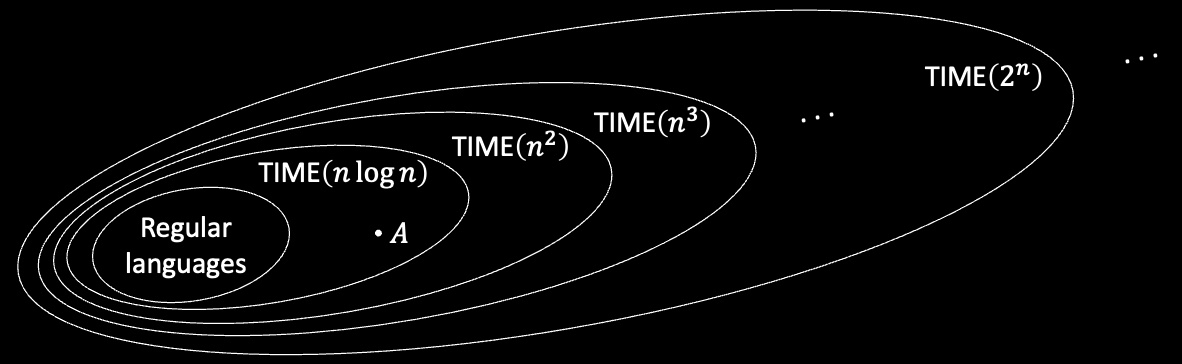
\includegraphics[width = \textwidth]{l12.1.jpg} 
    \end{figure}

\end{example}

\begin{note}
    Is there gap between \(TIME(n log n)\)  and \(TIME(n)\)? 

    This will be answered later in \textbf{Time Hierarchy Theorem}.  
\end{note}
\begin{problem}
    Let \(B = \{ww^R | w \in \{a, b  \}^*  \} \), what's the smallest function \(t\) that \(B \in TIME(t(n))\)?
    
    \begin{remark}
        \(ww^R\) means the right part is the reverse of the left part.
    \end{remark}

    Correct answer is \(O(n^2)\). 
\end{problem}

\section{Multi-tape vs 1-tape}
\begin{theorem}
    Let \(t(n) \geq n\).

    If a multi-tape TM decides \(B\) in time \(t(n)\), then \(B \in TIME(t^2(n))\).   
\end{theorem}
\begin{proof}
    Analysis conversion of multi-tape to 1-tape TMs.

    To simulate 1-step of \(M\)'s computation, \(S\) uses \(O(t(n))\) steps. 
    (\(S\)  stores multiple tapes in 1-tape and it has to move back and forth).

    So total simulation time is \(O(t(n) \times t(n)) = O(t^2(n))\) 
\end{proof}

\begin{definition}[polynomially related]
    Two models of computation are \underline{polynomially related} if each can simulate the other with a polynomial overhead:

    So \(t(n)\) times \(\rightarrow t^k(n)\) time on the other model, for some \(k\).   
\end{definition}

All reasonable deterministic models are polynomially related.

\begin{itemize}
    \item 1-tape TMs
    \item multi-tape TMs
    \item multi-dimensional TMs
    \item random access machine (RAM)
    \item cellular automata
\end{itemize}

\section{The Class P}

\begin{definition}[Defnition of P]
    \textbf{P} is the class of languages that are decidable in polynomial time on a deterministic string-tape TM:

    \(P = \bigcup_{k} TIME(n^k)\) = Polynomial time decidable languages
\end{definition}

Why \textbf{P} is important: 
\begin{itemize}
    \item Invariant for all reasonable deterministic models.
    \item Corresponds roughly to realistically \textbf{solvable} problems. (For example, not safe for cryptography)
\end{itemize}

\begin{example}
    \(PATH = \{ \langle G, s, t \rangle | G \) is a directed graph with a path form \(s\) to \(t\)  \}

    \begin{theorem}
        \(PATH \in P\) 
    \end{theorem}
    \begin{proof}
        \(M\) making all the nodes until nothing new can be marked. 

        Accept if \(t\) is marked, reject if not. 
    \end{proof}
\end{example}

\begin{example}
    \(HAMPATH = \{\langle G, s, t \rangle  | G\) is a\\ directed graph with a path from \(s\) to \(t\) and the \underline{path goes through every node of G}\}

    (This path is also called \textbf{Hamiltonian Path}).


    \begin{problem}
        \(HAMPATH \in P\)? 

        \begin{remark}
            This is a famous unsolved problem, equal to \(N = NP\) 
        \end{remark}
    \end{problem}

\end{example}

\section{Other examples}

\begin{theorem}[Thoream 7.16 in the book]
    Every context-free language is a member of P.
\end{theorem}